\subsection{Deep Q-Learning Agent}

In this section we are giving an overview of the experiments we have done with our deep q-learning model that lead to our best performing agent. The basic framework is already described in the sections Methods and Training (give reference here). Hence at this point we trained the model, evaluated the performance and based upon that we changed hyperparameters or auxiliary rewards to improve the model. We always conducted a similar training routine, namely starting off with a small field with height and width 7 containing coins on every tile, so 21 coins in total. This gave us the opportunity to already evaluate if there are flaws in the implementation or how fast the network converges with the chosen hyperparameters. Then we scaled the field up to 11 $\times$ 11 and increased the difficulty by including crates. Finally the agent was trained with all settings as in the target field, so a 17 $\times$ 17 field, 9 coins and a crate density of 0.75. The last step was to add opponents to train in the exact same environment our agent will be tested in. Simultaneously to raising size and difficulties we also increased the steps per round from 60 to 200, as the agent does not need 200 steps to collect all coins in a field as small as 7 $\times$ 7. (EVTL. SOLLTE DAS IN TRAININGS PART)

Initially most experiments resulted in the fine tuning of the rewards and auxiliary reward functions. A good indication that the rewards were not helping the model to get trained in the most efficient way was a big deviation between the sum of the rewards in comparison to the score achieved by the agent. Ideally the score in the end of a round is constantly quite high if the sum of the rewards is high, especially if the sum is in a high range after each round for many rounds already, so if it is converged. The plots in Figure \ref{fig:rewardVSscore} show an example of this phenomenon when the model was trained for 10000 rounds in the 7 $\times$ 7 coin-heaven scenario with coins on every tile . There is a quite sudden improvement in the score between the 2000th and 3000th round of training and this jump can also be observed in the rewards plot on the left but is much less significant. Furthermore the rewards plot still increases and seems to have converged after the 5000th round of training. Nonetheless the score is getting worse and keeps fluctuating between the highest possible score 21 and a score as low as 3. When letting the agent play we noticed that this happened because the agent dropped many unnecessary bombs and thus killed itself occasionally, so the agent was not able to collect all the coins. However the total amount of rewards was still high because the agent was rewarded a lot for outrunning a bomb and was not punished for dropping a totally unnecessary bomb. To understand this kind of behavior the logged messages were really helpful. Therefore we fine tuned the rewards with a closer examination of matching the extent of rewards for different actions with each other. We also added a penalty for dropping bombs that will not destroy crates or are in reach of an opponent. 
\begin{figure}[H]
    \centering
    \begin{minipage}{0.49\textwidth}
		\centering
		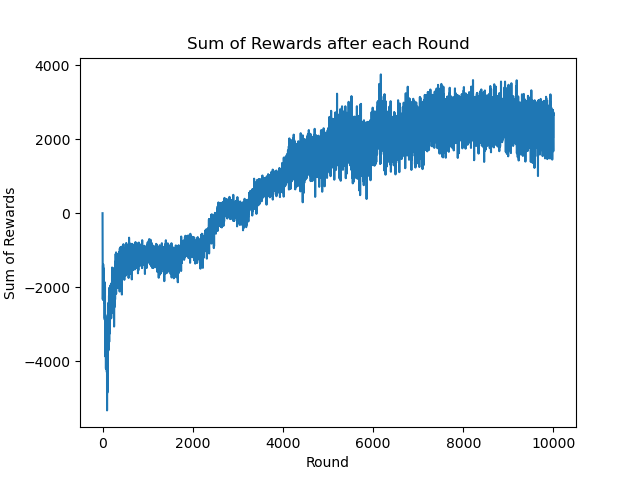
\includegraphics[scale=0.52]{images/rewards_converged.png}
    \end{minipage}
    \begin{minipage}{0.49\textwidth}
	\centering
		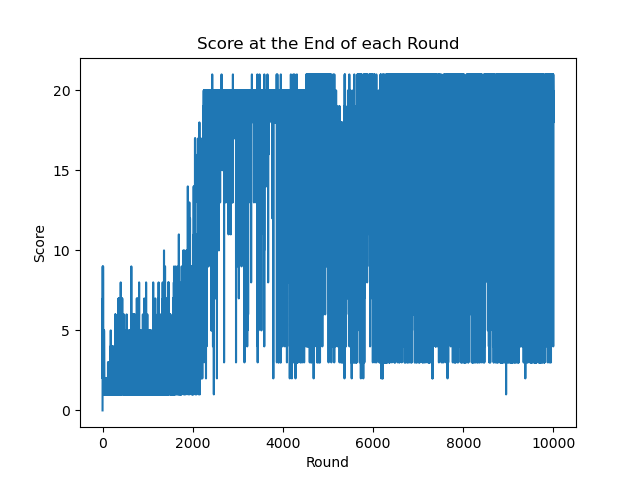
\includegraphics[scale=0.52]{images/scores_not_converged.png}
    \end{minipage}
    \caption{Both plots were generated during the training of the Deep Q-Model on a small coin-heaven scenario with coins on every free tile. The x-axis of both plots represent the rounds of the training. While the left plot depicts the sum of all rewards given to the agent in each round, the right plot shows the score after each round. These plots show discrepancy between rewards and scores.}
    \label{fig:rewardVSscore}
\end{figure}

After a little bit more trial and error and some more improvements of the rewards we were already able to produce a model that collected all coins efficiently. Figure \ref{fig:efficientCoinHeaven} shows the corresponding rewards and scores of 8000 rounds of training. This time score and reward coincide very well. Again between the 2000th and 3000th round the agent makes a jump and apparently found a good way to handle this environment. Henceforward, both scores and rewards, are on a constantly high level. Of course there is a certain amount of fluctuation as the agent is supposed to do some random moves during training to find a potentially better way of playing. Here the probability of doing a random move during training, not calculated by the network, was constantly 10\%.
\begin{figure}[H]
    \centering
    \begin{minipage}{0.49\textwidth}
		\centering
		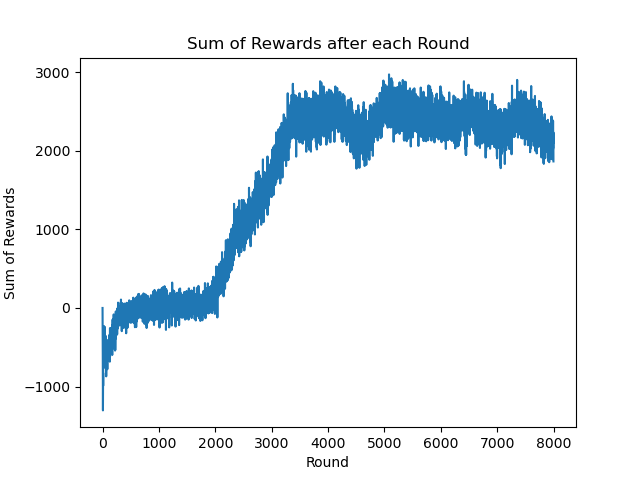
\includegraphics[scale=0.52]{images/rewards_perfect_coinheaven.png}
    \end{minipage}
    \begin{minipage}{0.49\textwidth}
	\centering
		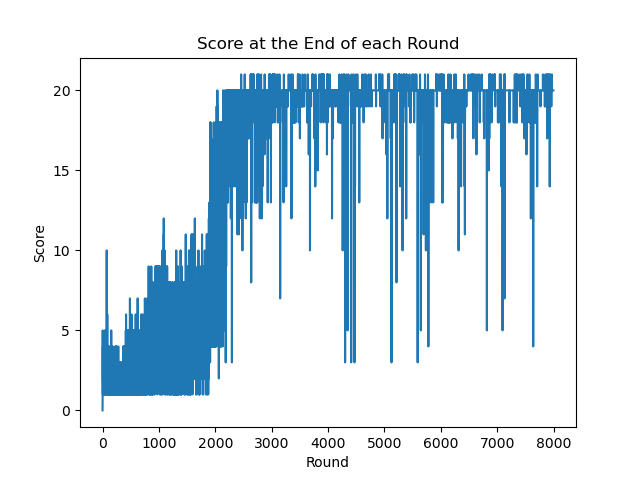
\includegraphics[scale=0.52]{images/scores_perfect_coinheaven.png}
    \end{minipage}
    \caption{The plots are constructed in the same way as before, but after reward fine-tuning the scores shown here fit to the high reward sum.}
    \label{fig:efficientCoinHeaven}
\end{figure}

Although the auxiliary reward functions seemed to be elaborated very well at this point the agent did not play smoothly on larger fields and in the harder levels even after a lot of training rounds. The main concern was that the agent often kept killing itself in early steps of the game. With the assumption that the rewards are given reasonably we also had to evaluate other hyperparameters. Our neural network consisted of a very simple architecture so we thought about features to add to the network to enable better learning. Even though dropout is a very common thing to have in neural networks, it did not make sense for our task as it is used to prevent overfitting, which cannot happen here. Instead we included batch normalization which should stabilize and accelerate the training. Unfortunately when doing the training from scratch the batch normalization did not result in a better running agent or a faster training, probably because the batch size was too small. Not only was the batch size small in general with 256, but we could not collect enough training samples if the agent killed itself early in the game. This did not allow the positive effects of batch normalization to unfold in our network.

Next we gave different loss functions a try. We initially used the smooth L1 loss but also thought of trying the cross-entropy loss because it is the standard loss for classification models, where the output usually is a list of probabilities. In our case the output gives the probability of the action to be the best action to take in the current state of the game for every possible action. Applying the cross-entropy loss showed that our model is not suited for this kind of loss. A reason for this could be that we want to find a good metric to calculate the loss between the predicted and the target q value, calculated following the Bellman equation. The literature hints that we should minimize the quadratic error between those values. In the formula for the cross-entropy loss the quadratic error is never calculated. Instead losses that can be considered next to the Smooth L1 loss is the closely related Huber loss and of course the MSE (mean squared error) loss. In the end MSE loss proofed to be most efficient, so our final agent was also trained with this loss. When discussing the loss we also inevitably gave thought to the optimizer. The AdamW optimizer worked well but RMSprop was more effective. Especially the faster convergences shown in Figure \ref{fig:adamvsrmsprop} was a decisive point in favor for the RMSprop optimizer. Thus we proceeded with RMSprop but as AdamW achieved good results too we believe that it would haven been able to run similarly when giving more consideration to the learning rate.
\begin{figure}[H]
    \centering
    \begin{minipage}{0.49\textwidth}
		\centering
		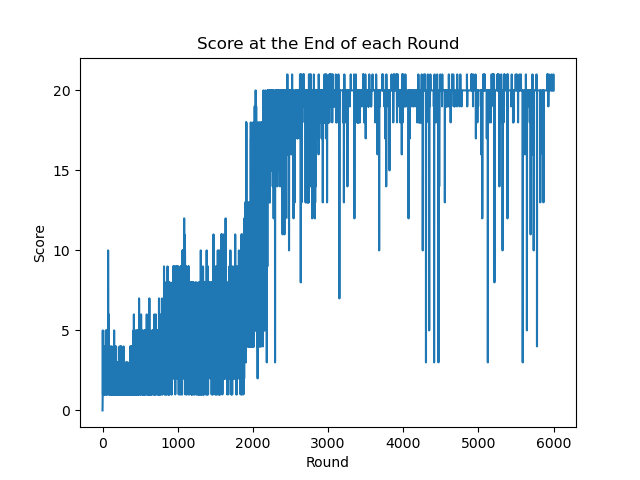
\includegraphics[scale=0.52]{images/scores_adamw.png}
    \end{minipage}
    \begin{minipage}{0.49\textwidth}
	\centering
		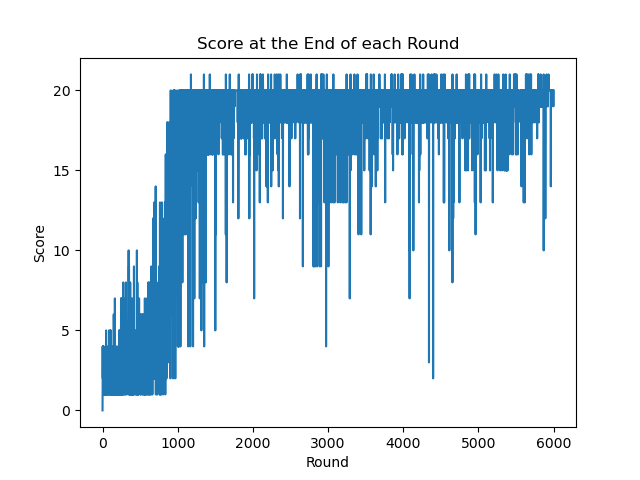
\includegraphics[scale=0.52]{images/scores_rmsprop.png}
    \end{minipage}
    \caption{The plots are constructed in the same way as before, but both plots depict the scores of to different trainings. The left one was trained with the optimizer AdamW and the right one was trained with RMSprop. The model using RMSprop improves and converges faster.}
    \label{fig:adamvsrmsprop}
\end{figure}

With the configurations chosen as explained above we reached a fairly good playing agent after 6000 rounds of training in coin-heaven (7 $\times$ 7 field, coins on every free tile and 60 steps per round), 60000 rounds of training in loot-crate (11 $\times$ 11 field, 20 coins, 0.4 crate density, 120 steps per round), 15000 rounds of training in classic (17 $\times$ 17 field, 9 coins, 0.75 crate density, 200 steps per round) and 40000 rounds of training in the classic scenario as described before but with two rule based agents and one coin collector agent as opponent. Strangely, except of being able to play the game well the agent did not learn to not do invalid actions. We observed that the majority of self killing happened because the agent still did invalid action, like trying to move in a direction where a wall is located to escape a bomb. Thus to get a better playing agent we forced the agent to not do invalid actions in the not-training mode. After each model output we check if the chose action, so the action with the highest probability, is possible and if not we take the action with the second highest probability and check this one and so on. 

Finally, we created an agent that can compete with a rule based and coin collector agent but is mostly not able to beat them. Still we can conclude that our model did learn how to play the game as it clearly outperforms a random agent, which nearly always makes 0 points. Figure \ref{fig:game1} shows the scores of four agents, namely our reinforcement learning agent, a rule based agent, a coin collector agent and a random agent, when they play against each other in the classic scenario for 10 rounds. We also found that our agent performs better against stronger agents, maybe because it was trained against strong agents. When we chose the same opponents as during training, so 2 rule based agents and 1 coin collector, our agent often outperforms at least one of them.
\begin{figure}[H]
    \centering
    \begin{minipage}{0.49\textwidth}
		\centering
		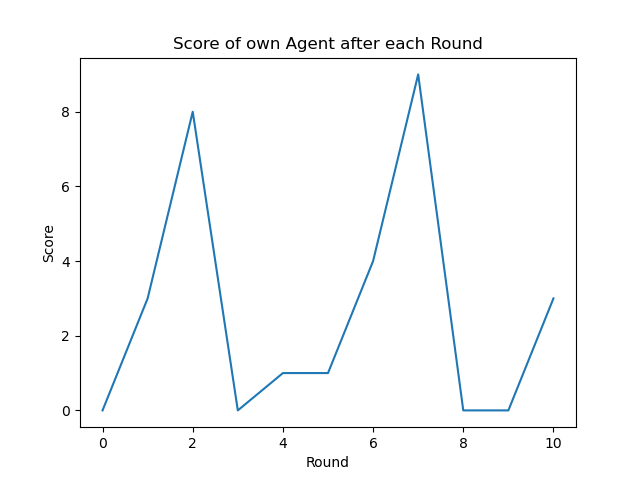
\includegraphics[scale=0.52]{images/my_scores11_1.png}
    \end{minipage}
    \begin{minipage}{0.49\textwidth}
	\centering
		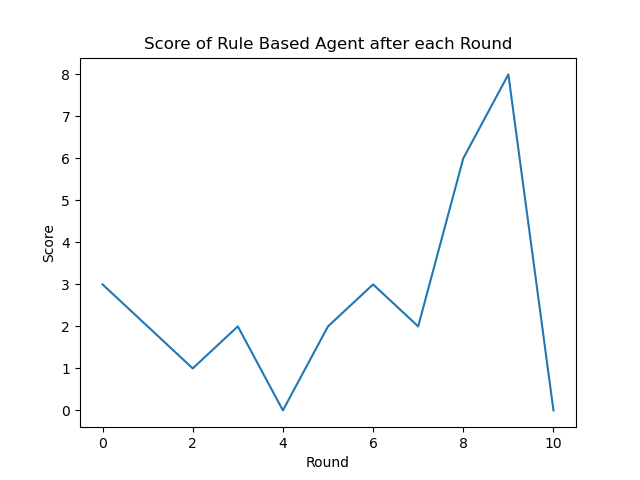
\includegraphics[scale=0.52]{images/rule_scores11_1.png}
    \end{minipage}
    \begin{minipage}{0.49\textwidth}
		\centering
		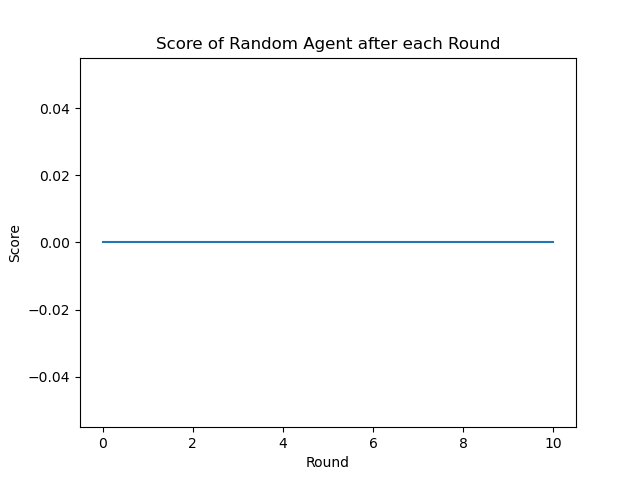
\includegraphics[scale=0.52]{images/random_scores11_1.png}
    \end{minipage}
    \begin{minipage}{0.49\textwidth}
	\centering
		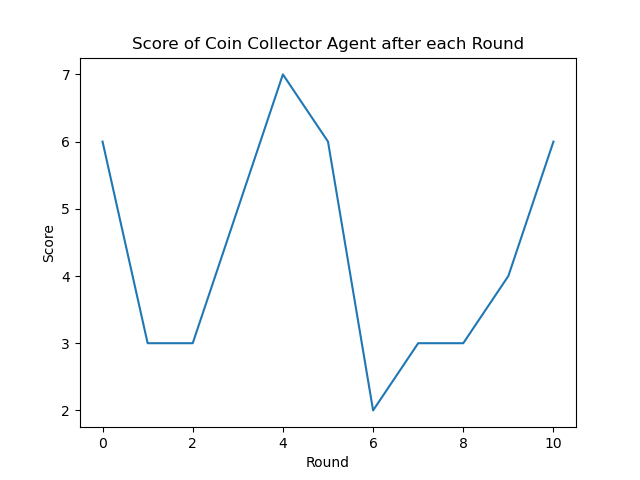
\includegraphics[scale=0.52]{images/coin_scores11_1.png}
    \end{minipage}
    \caption{These plots result from one game of bomberman with 10 rounds. Our reinforcement learning agent played against a rule based agent, a coin collector agent and a random agent. While the random agent did not score any points, our agent and the rule based agent both scored 29 points in total and the coin collector won with 46 points.}
    \label{fig:game1}
\end{figure}

notes:

%- this is the part where we trained, evaluated and then changed hyperparameters or even tried to improve our auxiliary rewards\\
%- conducted training always similar, started off with only coins, then with crates, then with opponents, not only harder enivronments but also got bigger from 7x7 to 11x11 to 17x17 (probably mention that already in Training section)\\
- 2 Aufteilungsmöglichkeiten, entweder wie die unterschiedlichen optimierungen vom trainingslevel her waren, also aufteilen in coins, crates und opponent training und verbesserungen oder für jede Trainingsänderung\\
%- in the beginning most of the experiments let to fine tuning of the auxilary rewards: e.g after training in coin heaven look at difference between the high constantly high reward and very fluctuating score (plots:Git3, destroyer of universes, neuer reward, 1.Training)\\
- of course in training should be some randomness but the low score came from the agent killing itself which was due to dropping many unnecessary bombs because outrunning the bomb was more effect in regards to the rewards than only collecting the coins\\
- in coin heaven scenario with 7x7 field left a nearly perfect result, where the agent collects all coins very efficiently, also shown in plots (Git3, destroyer of universes, neuer reward 5, 1. Training)\\
- in these plots we can also see a clear point where the agent, randomly picked a very good path and kept improving on that till final converging, except some outliers due to randomly chosen action in training\\
- at this point the probability for randomly chosen action was constant at 10\%\\
- took logs as help to understand what happend during training, and what the agent learned to do because of the rewards\\
- although at this point the rewards seemed pretty good there were troubles when going into the bigger training scale with crates and opponents and bigger fields\\
- one of our main concerns was the fact that the agent killed himself very often, and sometimes quite early (plots rewards 5, 12. Training, clarify that this was not only training, but the last 10000 rounds of training), again very flactuating, basically only 0 score so often because killing self before getting the chance to collect many coins\\
- when assuming that the rewards are given in a way that enables the agent to learn the game efficiently, we had to evaluate other hyperparameters and check if they enable better and more learning\\
- a very basic nn architecture, common features to add in nn is e.g. dropout but as this is to prevent overfitting, which is not a problem in reinforcement learning we didn't apply that\\
- batch norm unfortunately didn't do anything for us at the point we tested it, which probably was caused by too low batch sizes in general but especially because the batch size also depended on the amount of rounds saved in our memory class, and if the agent killed in itself early the batch probably was as small as 3 samples, question is would batch norm give us a big advantage anyway, as it is more helpful in deep networks to stabilize and make the training faster \\%(https://towardsdatascience.com/batch-normalization-in-3-levels-of-understanding-14c2da90a338#3164)
- we added batch norm before addition of the multiple models and before activation as suggested by \\%(http://torch.ch/blog/2016/02/04/resnets.html)
- loss initially started with smooth l1 closely related to huber, also tested huber which converges to mse loss which worked very well (the final agent was trained with mse loss but a very similar result would probably also be possible with huber/smoothl1), cross entropy was not working very well, literature says squared loss of target q and predicted q value\\ %smooth vs huber https://pytorch.org/docs/stable/generated/torch.nn.SmoothL1Loss.html %https://medium.com/intro-to-artificial-intelligence/deep-q-network-dqn-applying-neural-network-as-a-functional-approximation-in-q-learning-6ffe3b0a9062#:~:text=In%20a%20DQN%2C%20we%20can,value%20and%20prediction%20Q%20value.&text=In%20DQN%2C%20we%20make%20use,of%20the%20Q%2Dlearning%20algorithm.
- optimizer adamw was effective, rmsprop in combination with mse loss showed the best results and also faster convergence, maybe if fitting learning rate better adamw would be able to come up with same results, convenient not to bother with the learning rate (plots Git 3 mse rms 1. Training vs reward 5 1. Training, schnellere konvergenz in scores, ähnlich für rewards)\\
- excluded invalid actions because logs showed that this happens when trying to escape bomb, agent should be able to learn this (cannot go into walls) but we definitely want to avoid it even if it is not learned (create plots of agent that avoids invalid action vs not avoids invalid actions)\\
- batch norm, loss (huber, cross entropy, mse, smmothl1), optimizer changed (AdamW vs RMSProp), excluding invalid action in play modus (not during training), more memory, batch size (256) and randomness threshold calculated dependent on round (unfortunately detected error very late, that it was dependent of step in round instead of round, so did it manually, starting with hihger probability like 0.1 and going down to 0.05 and 0.025)\\
-plots final one running against random and rule based (maybe already do that earlier, as proof that we are on right track)